\section{Project Plan}

\subsection{Resources}

\begin{enumerate}
    \item 1 Data Scientist: Miguel Tablado will be playing this role and will dedicate 300h
    \item 1 Coach/Tutor: Baris Kanber will be supervising Miguel Tablado during the project
    \item MRI images and demographic information from IXI Dataset
    \item GPU resources are needed to train and test the network
\end{enumerate}

\subsection{High Level Plan}

The plan will be executed in 3 different phases with the listed tasks:
\begin{enumerate}
    \item Phase 1: Analysis
    \begin{enumerate}
        \item Gain knowledge on MRI and NIFTI protocol
        \item Describe images and dataset
        \item Extract 2D images
        \item Pre-processing images
    \end{enumerate}
    \item Phase 2: MR Images creation
    \begin{enumerate}
        \item Test different Network architectures
        \item Tune-up architectural network
    \end{enumerate}
    \item Phase 3: Project documentation
    \begin{enumerate}
        \item Write conclusions
        \item Create project documentation
        \item Create project presentation
    \end{enumerate}
\end{enumerate}

\begin{figure}[ht]
    \centering
    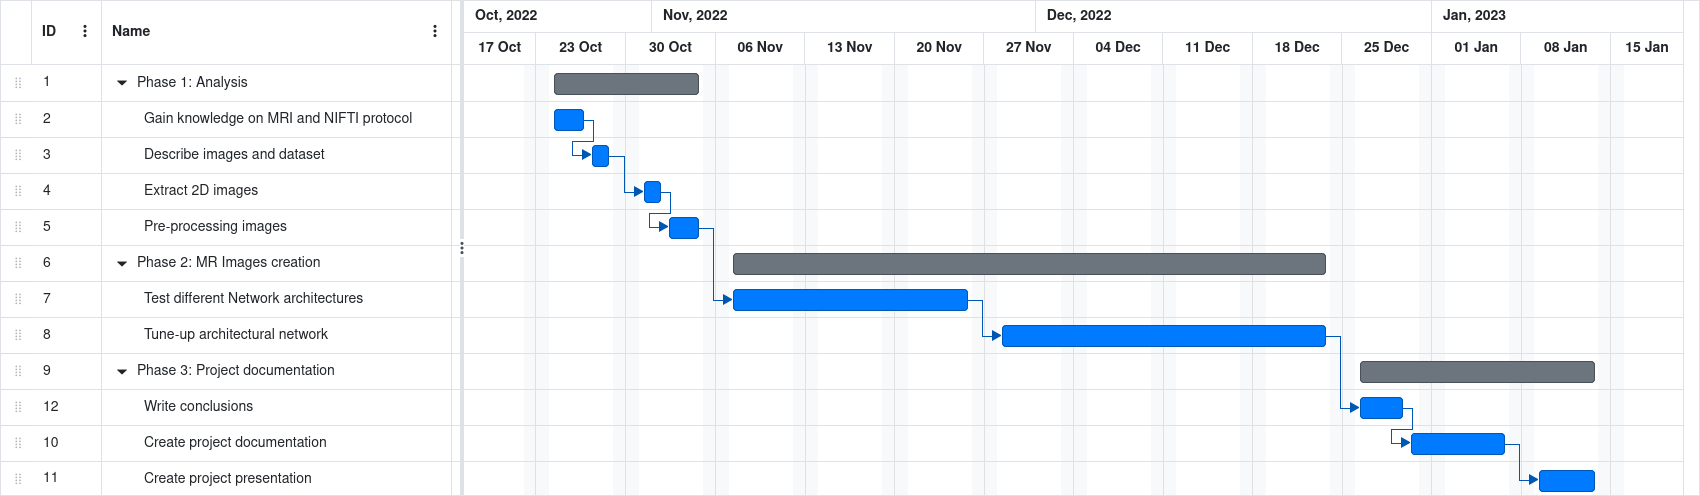
\includegraphics[width = 17cm, height = 6cm]{images/project-plan.png}
    \caption[Project Plan]{Project Plan. Created using: https://www.onlinegantt.com}
    \label{fig:project-plan}
\end{figure}

\newpage
\subsection{Tasks}
\subsubsection*{Phase 1: Analysis}

During this phase the different tasks will be executed to prepare the work and includes:
\begin{enumerate}
    \item Gain knowledge on MRI and the NIFTI file format: This activity consists of reading papers and documents to gain sufficient knowledge to execute the project. There is no need to become an expert on the matter but understanding how those files are and how to process them.
    \item Describe images and dataset: During this activity, a description of the dataset will be generated with a view of the quality of the dataset for the aim of the project and any findings which could result.
    \item Extract 2D images: Load 3D images and extract 2D slices from the original dataset, which will be depicted with code.
    \item Pre-processing images: Decide which transformations on the 2D images would help the project like pixel changes or applying gray-scale transformations.
\end{enumerate}

\subsubsection*{Phase 2: MR Images creation}

\begin{enumerate}
    \item Test different Network architectures: This task will take few existing network architectures and be tested with the dataset so that one of them will be selected to be improved and used as the project architecture.
    \item Tune-up architectural network: Tune the selected architecture with useful techniques like changing network layers
\end{enumerate}